\chapter{CR power plant simulation}
%For the CR plant simulation in SAM, the \enquote{CSP power tower molten salt} model was selected. To specify the hourly atmospheric conditions the EPW weather file for Upington from Section~\ref{Solar radiation} was used as an input file. As already mentioned, the LCOE was calculated separately using a simplified method which is documented in Appendix~\ref{ChapterLCOE} on Page \pageref{ChapterLCOE}.
For the CR plant simulation in SAM, the \enquote{CSP power tower molten salt} model was selected. To specify the hourly atmospheric conditions, the EPW weather file for Upington from Section~\ref{Solar radiation} was used as an input file. As already mentioned, the LCOE was calculated separately using a simplified method.

\section{Design and simulation} \label{CR power plant design  and simulation}
%This section describes in detail the crucial inputs of the CR power plant components, namely the power cycle, heliostat field, tower and receiver and thermal energy storage (TES), as well as there individual financial parameter.

%The simulated configurations were to meet 90~\% of the scheduled production curve by using variation of solar multiples and full load hours of TES. As mentioned in Section~\ref{Large scale concentrated solar power (CSP) plants} the solar multiple (SM) is the ratio of the receiver's thermal output to the power cycles thermal input at the design point. Thus, a CR system with a SM of 1 has a receiver and a heliostat field which provides the thermal power needed for the power block to run at full load at the system design point. A receiver and collector field with an SM of 1 do not produce enough thermal power to store energy in a TES while also feeding the turbine. A CR system with a SM of 1 is just sufficient for systems without TES. In order to cover the expected load, the solar multiple was varied from 2 to 3.5 in steps of 0.5, while storage full load hours were varied from 8 to \SI{16}{h} in steps of \SI{2}{h}. The target of \SI{100}{MW} net capacity was reached with a gross capacity of \SI{111}{MW} with an estimated gross-to-net conversion of \SI{90}{\percent}. Table~\ref{tbl: CR_OverallConfig} summarizes the simulated configurations.

The simulated configurations were to meet \SI{90}{\percent} of the prescribed load profile by using variation of solar multiples and full load hours of TES. A CR system with a SM of 1 has a receiver and a heliostat field which provides the thermal power needed for the power block to run at full load at the system design point. A receiver and collector field with an SM of 1 do not produce enough thermal power to store energy in a TES while also feeding the turbine. A CR system with a SM of 1 is just sufficient for systems without TES. In order to cover the expected load, the solar multiple was varied from 2 to 3.5 in steps of 0.5, while storage full load hours were varied from \num{8} to \SI{16}{h} in steps of \SI{2}{h}. The target of \SI{100}{MW} net capacity was reached with a gross capacity of \SI{111}{MW} with an estimated gross-to-net conversion of \SI{90}{\percent}. Table~\ref{tbl: CR_OverallConfig} summarizes the simulated configurations.

\begin{table}[!h]  
  \centering
	\begin{tabular}{ p{4.0cm}  C{1.0cm} C{0.3cm} C{0.3cm} C{0.3cm} C{0.3cm} C{0.3cm} | C{0.3cm} C{0.3cm} C{0.3cm} C{0.3cm} C{0.3cm} } 
	\hline	
\textbf{Item} & \textbf{Unit} & \multicolumn{10}{c}{\textbf{Value}} \\ \hline \hline
Net turbine capacity & \si{\mega\wattel} & \multicolumn{10}{c}{100} \\
Gross turbine capacity & \si{\mega\wattel} & \multicolumn{10}{c}{111} \\ \hline
Solar multiple & - & \multicolumn{5}{c}{2.0} & \multicolumn{5}{c}{2.5} \\
TES capacity & h &  8 & 10 & 12 & 14 & 16 &  8 & 10 & 12 & 14 & 16 \\ \hline 
Solar multiple & - & \multicolumn{5}{c}{3.0} & \multicolumn{5}{c}{3.5} \\
TES capacity & h &   8 & 10 & 12 & 14 & 16 &  8 & 10 & 12 & 14 & 16 \\ \hline 
\end{tabular}
\caption[Simulated CR solar multiple and thermal energy storage configurations.]{Simulated CR solar multiple and thermal energy storage  configurations.}\label{tbl: CR_OverallConfig}
\end{table}
\subsubsection{Power cycle}
%The power cycle of the simulated CR system features a Rankine-cycle steam engine, two open feed-water heaters, a pre-heater, boiler and super-heater \cite{NREL2015a}. As mentioned above has the turbine a gross capacity of \SI{111}{\mega\wattel} and a nameplate (net) capacity of 100 \si{\mega\wattel}. 

The power cycle of the simulated CR system features a Rankine-cycle steam engine, two open feed-water heaters, a pre-heater, boiler and super-heater \cite{NREL2015a}. The turbine has a gross capacity of \SI{111}{\mega\wattel} and a nameplate (net) capacity of 100 \si{\mega\wattel}. 

%The steam generator has a HTF inlet temperature of \SI{566}{\celsius} and outlet temperature of \SI{288}{\celsius} at design point and operates at a pressure of \SI{125}{\bar}. In combination with a air-cooled condenser the CR power cycle system was simulated with a cycle gross efficiency of \SI{41.2}{\percent}. A wet-cooled condenser would reaches some higher efficiency, but because of the lack of water in the area of Upington and the requirement by the South African government for CSP plants, a air-cooled condenser was selected. The HTF inlet temperature, pressure and efficiency values where adapted for the configuration from \cite{Kolb2011a}. For starting up the system needs 30 minutes and a min. required temperature of \SI{500}{\celsius}. A plant availability of 96~\% was adapted from \cite{Morin2012} in order to simulate system down-times for outages or scheduled maintenance.

The steam generator has an HTF inlet temperature of \SI{566}{\celsius} and outlet temperature of \SI{288}{\celsius} at design point and operates at a pressure of \SI{125}{\bar}. In combination with an air-cooled condenser, the CR power cycle system was simulated with a cycle gross efficiency of \SI{41.2}{\percent}. A wet-cooled condenser would achieve higher efficiency, but because of the lack of water in the area of Upington and government requirements for CSP plants, an air-cooled condenser was selected. The HTF inlet temperature, pressure and efficiency values where adapted for the configuration from \cite{Kolb2011a}. At start-up, the system needs 30 minutes and a minimum temperature of \SI{500}{\celsius}. A plant availability of \SI{96}{\percent} was adopted from \cite{Morin2012} in order to simulate system down-times for outages or scheduled maintenance.

\begin{table}[!h]  
  \centering
	\begin{tabular}{  p{7.0cm}  C{2.0cm}  C{2.0cm} } 
	\hline	
\textbf{Item} & \textbf{Value} & \textbf{Unit} \\ \hline \hline
Turbine design capacity, gross  & \num{111} & \si{\mega\wattel} \\ 
Turbine design capacity, net & \num{100 }& \si{\mega\wattel} \\ 
Boiler operating pressure & \num{125}& bar \\ 
Design inlet temperature & \num{288}& \si{\celsius} \\ 
Design outlet temperature & \num{566}& \si{\celsius} \\ 
Cycle conversion efficiency & \num{41.2} & \% \\ 
Steam generator design thermal power & \num{269.42} & \si{\mega\wattth}  \\
Power block start-up time & \num{0.5} & h \\ 
Minimum required start-up temperature & \num{500} & \si{\celsius} \\
Plant availability  & \num{96} & \\
Condenser type & air-cooled & - \\ 
\hline
\end{tabular}
\caption[CR power block and condecer input parameter in SAM.]{CR power block and condecer input parameter in SAM.}\label{tbl: CRPowerplant}
\end{table}
\subsubsection{Heliostat field}
%The heliostat field design was done in SAM using its heliostat field layout optimization tool. For the design, optimization and simulation process, heliostat data from the Sanlúcar 120 heliostat was used \cite{Noone2012}. The Sanlúcar 120 is used in the Planta Solar 10 (PS10) near Seville, Spain and is the origin of Abengoas actual heliostat ASUP 140. For a simulation with the ASUP 140 no sufficient data was available. 
The heliostat field design was done in SAM using its heliostat field layout optimization tool. For the design, optimization and simulation process, heliostat data from the Sanlúcar 120 heliostat was used \cite{Noone2012}. The Sanlúcar 120 is used in the Planta Solar 10 (PS10) near Seville, Spain and is the predecessor to the Abengoas ASUP 140 heliostat. For a simulation with the ASUP 140, no data was available.

\begin{table}[!htbp]  
  \centering
	\begin{tabular}{ p{4.5cm}  C{1.5cm} C{1.2cm} C{1.2cm} C{1.2cm} C{1.2cm} } 
	\hline	
\textbf{Item} & \textbf{Unit} & \multicolumn{4}{c}{\textbf{Value}} \\ \hline \hline
racking & - &  \multicolumn{4}{c}{two-axis} \\
Height & m  &  \multicolumn{4}{c}{\num{9.45}} \\
Width & m  &  \multicolumn{4}{c}{\num{12.84}} \\
Reflective area & \si{\square\metre} &  \multicolumn{4}{c}{\num{120.00}} \\
Heliostat availability& \% &  \multicolumn{4}{c}{\num{99}} \\
Design-point DNI & \si{\watt\per\square\metre} &  \multicolumn{4}{c}{\num{950}} \\
\hline
\textbf{Solar multiple}& \textbf{-} & \textbf{2.0} & \textbf{2.5} & \textbf{3.0} & \textbf{3.5}\\ \hline 
Number of heliostats & - & \num{9131} & \num{11530} & \num{13976} & \num{16658} \\
Max. distance from tower & m & \num{1528} & \num{1708} & \num{1883} & \num{2010} \\
Reflective area  & ha & \num{109.58} & \num{138.36} & \num{167.72} & \num{199.90} \\
Field land area & ha & \num{655.59} & \num{821.92} & \num{997.95} & \num{1190.99} \\ 
\hline
\end{tabular}
\caption[CR heliostat parameters.]{CR heliostat parameters.}\label{tbl: CRHeliostats}
\end{table}
%The Sanlúcar 120 heliostats have an effective reflective area of \SI{120}{\square\metre} and are tracked on 2 axes. The heliostat field layout optimization and there design depends on the turbine gross and the SM. The heliostat field was optimized therefore for all four considered configurations. SAM first generates a coarse layout and optimizes the number of heliostats and their position. The goal of the optimization is the maximum flux with minimum power constraints according to the specified design-point DNI which represents the DNI at which the power plant achieves its rated thermal capacity. Table~\ref{tbl: CRHeliostats} summarizes the heliostat datas and the values of the optimized field design for all considered solar multiples.

The Sanlúcar 120 heliostats have an effective reflective area of \SI{120}{\square\metre} and are tracked on 2 axes. The heliostat field layout optimization and design depends on the turbine gross and the SM. The heliostat field was optimized for all four considered configurations. SAM first generates a coarse layout and optimizes the number of heliostats and their position. The goal of the optimization is the maximum flux with minimum power constraints according to the specified design-point DNI, which is the DNI at which the power plant achieves its rated thermal capacity. Table~\ref{tbl: CRHeliostats} summarizes the heliostat datas and the values of the optimized field design for all considered solar multiples.

%The optimized heliostat field layouts which was used in the simulation can be seen in Appendix~\ref{documentary} on Page~\pageref{SM}.
The optimized heliostat field layouts which were used in the simulation can be seen in Appendix~\ref{documentary}, page~\pageref{SM}.

\subsubsection{Tower and receiver}
%The receiver collects the concentrated irradiance from the surrounding heliostat field. The simulated receiver is build as an external cylindrical receiver and is configurated with 24 panels of thin walled (1.25 mm) receiver tubes with an outer diameter of 60 mm arranged in a circle around the tower. The receiver tubes are made from 316H stainless steel and the external surfaces of the tubes are coated with a black Pyromark paint. The paint is resistant to high temperatures and thermal cycling, and absorbed 95\% of the incident sunlight. This configuration is similar to the receiver of the  Solar Two Project accept of the outer diameter \cite{Bradshaw2002}. The panels containing molten salt (60~\% NaNO\textsubscript{3} and 40~\% KNO\textsubscript{3}) as heat transfer fluid (HTF). The receiver design inlet temperature of 288$\,^{\circ}\mathrm{C}$ and the outlet temperature of 566$\,^{\circ}\mathrm{C}$ was set before in the power block configuration. In order to achieve the desired receiver thermal power output, the height of the tower and receiver dimensions got also adjust with the optimization of the heliostat field design. The results of the optimization is shown in Table~\ref{tbl: CRSolarfield}, as well as the fixed tower and receiver parameter. The heights of the tower range from 179.77 to \SI{236.50}{m}. The receiver proportions rises with the SM and the field sizes and results in a receiver thermal power range from 538.8 to 943.0 \si{\mega\wattth}.
The receiver collects the concentrated irradiance from the surrounding heliostat field. The simulated receiver is built as an external cylindrical receiver and is configured with 24 panels of thin walled (1.25 mm) receiver tubes, with an outer diameter of 60 mm arranged in a circle around the tower. The receiver tubes are made from 316H stainless steel and the external surfaces of the tubes are coated with black Pyromark paint. The paint is resistant to high temperatures and thermal cycling, and absorbs \SI{95}{\percent} of the incident sunlight. This configuration is similar to the receiver of the Solar Two Project, apart from the outer diameter \cite{Bradshaw2002}. The panels contain molten salt (\SI{60}{\percent} NaNO\textsubscript{3} and \SI{40}{\percent} KNO\textsubscript{3}) as heat transfer fluid (HTF). The receiver design inlet temperature of \SI{288}{\celsius} and the outlet temperature of \SI{566}{\celsius} was set before the power block configuration. In order to achieve the intended receiver thermal power output, the height of the tower and receiver dimensions were adjusted during the optimization of the heliostat field design. The results of the optimization along with the fixed tower and receiver parameters are shown in Table~\ref{tbl: CRSolarfield}. The heights of the tower range from \num{179.77} to \SI{236.50}{m}. The receiver proportion rises with the SM and the field sizes and results in a receiver thermal power range from 538.8 to \SI{943.0}{\mega\wattth}.


\begin{table}[!h]  
  \centering
	\begin{tabular}{ p{5.5cm}  C{1.5cm} C{1.2cm} C{1.4cm} C{1.4cm} C{1.4cm} } 
	\hline	
\textbf{Item} & \textbf{Unit} & \multicolumn{4}{c}{\textbf{Value}} \\ \hline \hline
Receiver configuration & - &  \multicolumn{4}{c}{external cylindrical receiver}\\
Heat transfer fluid & - &  \multicolumn{4}{c}{\SI{60}{\percent} NaNO\textsubscript{3} and \SI{40}{\percent} KNO\textsubscript{3}}\\
Inlet temperatures & \si{\celsius} &  \multicolumn{4}{c}{\num{288}}\\
Outlet temperatures & \si{\celsius} &  \multicolumn{4}{c}{\num{566}}\\
Receiver tube material & - &  \multicolumn{4}{c}{AISI316 stainless steel}\\
Receiver tube outer diameter & \si{\milli\metre} &  \multicolumn{4}{c}{\num{60}}\\
Receiver tube wall thickness & \si{\milli\metre} &  \multicolumn{4}{c}{\num{1.25}}\\
Number of panels & - &  \multicolumn{4}{c}{\num{24}}\\
Absorption factor  & - &  \multicolumn{4}{c}{\num{0.95}}\\
\hline
\textbf{Solar multiple} &  & \textbf{2.0} & \textbf{2.5} & \textbf{3.0} & \textbf{3.5}\\ \hline 
Tower height & \si{\metre} & \num{179.77} & \num{200.96} & \num{221.57} &  \num{236.50}\\
Receiver height  & \si{\metre} & \num{22.55} & \num{25.45} & \num{27.74} &  \num{29.94}\\
Receiver diameter & \si{\metre} & \num{14.85} & \num{16.66} & \num{17.91} & \num{18.77}\\ 
Receiver aperture area & \si{\square\metre} & \num{1052} & \num{1332} & \num{1561} & \num{1765} \\ 
Receiver thermal power & \si{\mega\wattth} & \num{538.8} & \num{673.5} & \num{808.3} & \num{943.0} \\
\hline
\end{tabular}
\caption[CR heliostat field parameters.]{CR heliostat field parameters.}\label{tbl: CRSolarfield}
\end{table}

\subsubsection{Thermal energy storage (TES)}
%The CR system was simulated using a direct two-tank molten salt thermal energy storage (TES). The storage uses directly the HTF (60~\% NaNO\textsubscript{3} and 40~\% KNO\textsubscript{3}) from the receiver as storage medium. Figure~\ref{towerdirecttwotank} on Page~\pageref{towerdirecttwotank} shows a schema of the direct storage for CR system. The design temperature of the hot storage tank (566$\,^{\circ}\mathrm{C}$) and the cold storage tank (288$\,^{\circ}\mathrm{C}$) depends also from the set value in the power block settings as before the design receiver temperatures. So the design temperature difference between the tanks is 278$\,^{\circ}\mathrm{C}$.

The CR system was simulated using direct two-tank molten salt thermal energy storage (TES). The storage takes the HTF (\SI{60}{\percent} NaNO\textsubscript{3} and \SI{40}{\percent} KNO\textsubscript{3}) directly from the receiver and uses it as the storage medium. Figure~\ref{towerdirecttwotank}, page~\pageref{towerdirecttwotank} contains a schematic of such direct storage for CR systems. The design temperature of the hot storage tank (\SI{566}{\celsius}) and the cold storage tank (\SI{288}{\celsius}) depends on the set value in the power block settings, just as in the receiver design. The design temperature differential is \SI{288}{\celsius}.

%As defined at the beginning of this Chapter, the full load hours of TES are varied in steps of \SI{2}{h} from 8 to \SI{16}{h}. The TES full load hours represents the time in which the storage can supply enough energy to the steam turbine and the power block to run at full design capacity. So a higher value of TES full load hours extended the time that the power plant can run during nights or cloudy days. Table~\ref{tbl: CRTES} shows that with higher TES full load hours the thermal capacity and tank volume increases as well. The simulated storage capacity is in a range of 2~\SI{155}{\mega\wattth\hour} using 8 full load hours and 4~\SI{311}{\mega\wattth\hour} using 16 full load hours. 

Full load hours of TES are varied in steps of \SI{2}{h} from 8 to \SI{16}{h}. The TES full load hours represents the time in which the storage can supply enough energy to the steam turbine and the power block to run at full design capacity, higher values extend the time the plant can run in darkness or under overcast conditions. With higher TES full load hours, the thermal capacity and tank volume increase as well (see Table~\ref{tbl: CRTES}). The simulated storage capacity is in a range of \SIrange{2}{155}{\mega\wattth\hour} using 8 full load hours and \SIrange{4}{311}{\mega\wattth\hour} using 16 full load hours.

\begin{table}[!h]  
  \centering
	\begin{tabular}{ p{3.9cm}  C{1.0cm} C{1.2cm} C{1.2cm} C{1.2cm} C{1.2cm} C{1.2cm} } 
	\hline	
\textbf{Item} & \textbf{Unit} & \multicolumn{5}{c}{\textbf{Value}} \\ \hline \hline
Storage type & - &  \multicolumn{5}{c}{direct two-tank molten salt}\\
Storage fluid & - &  \multicolumn{5}{c}{\SI{60}{\percent} NaNO\textsubscript{3} and \SI{40}{\percent} KNO\textsubscript{3}}\\
Hot tank design temp. & \si{\celsius} & \multicolumn{5}{c}{\num{566}}\\
Cold tank design temp. & \si{\celsius} & \multicolumn{5}{c}{\num{288}}\\
\hline
\textbf{TES full load hours} & \textbf{h} & \textbf{8} & \textbf{10} & \textbf{12} & \textbf{14} & \textbf{16}\\ \hline 
Thermal capacity & \si{\mega\wattth\hour} & \num{2155} & \num{2694} & \num{3233} & \num{3772} &  \num{4311}\\
Storage volume  & \si{\cubed\metre} & \num{10229} & \num{12787} & \num{15345} & \num{17902} & \num{20460}\\
\hline
\end{tabular}
\caption[CR system TES parameters.]{CR system TES parameters.}\label{tbl: CRTES}
\end{table}

%SAM 2015.6.30 r3 don't have a power control to follow prescribed hourly net output values. The turbine output of each day needs to be scheduled in front for the simulation. Thereby the parasitic consumer needs highly attention. The for the simulation designed scheduled turbine output matrix can be found in Appendix~\ref{documentary} on Page~\pageref{CR_turbineoutput}.

SAM 2015.6.30 r3 does not have a power control to follow prescribed hourly net output values. The turbine output of each day must be scheduled before the simulation, so particular attention must be paid to parasitic consumers. The turbine output matrix may be found in Appendix~\ref{documentary} on page~\pageref{CR_turbineoutput}.


\subsubsection{Financial parameters}
%The specific costs of the heliostat field of \SI{180}{\usd\per\square\metre} coming from J. B. Blackmon \cite{Blackmon2012}. He analyzed the costs of heliostat as a function of area for a representative solar central receiver power plant and calculated the total installed costs for a field of 5~000 heliostats with \SI{148}{\square\metre} reflective area of approximately \SI{180}{\usd\per\square\metre}. The analyze results showed that the costs are increasing with the size of the heliostats from \SI{40}{\square\metre} on. So the adopted value of \SI{180}{\usd\per\square\metre} reflective area for \SI{140}{\square\metre} heliostats can be assumed as conservative.

The specific costs for the heliostat field of \SI{180}{\usd\per\square\metre} are taken from J. B. Blackmon \cite{Blackmon2012}. He analyzed the costs of heliostats as a function of area for a representative solar central receiver power plant and calculated the total installed costs for a field of \num{5000} heliostats with \SI{148}{\square\metre} reflective area to be approximately \SI{180}{\usd\per\square\metre}. In his analysis, the costs increased with the size of the heliostats starting at \SI{40}{\square\metre}. So the adopted value of \SI{180}{\usd\per\square\metre} reflective area for \SI{140}{\square\metre} heliostats may be taken as conservative.

The remaining investment costs are based on the \enquote{Power Tower Technology Roadmap and Cost Reduction Plan} from 2011 \cite{Kolb2011}.

%On top of the investment costs a came 15 \% once-off surcharge for EPC and contingencies \cite{Platzer2014}.
A \SI{15}{\percent} one-off surcharge for EPC and contingencies was added on top of the investment costs \cite{Platzer2014}.

%Fichtner analyzed the annual O\&M costs with 1.84-1.96~\% of the total investment costs for CR power plants in SA \cite{Fichtner2010}. The value of \SI{2}{\percent} can so also be assumed as conservative.
Fichtner determined annual O\&M costs to be \SIrange{1.84}{1.96}{\percent} of the total investment costs for CR power plants in South Africa \cite{Fichtner2010}, so \SI{2}{\percent} may also be taken as conservative.

%The costs for the land purchase comes from the "African Agriculture Review" report of the Nedbank Capital, which reported the prices for farmland in SA. For the LCOE calculation of the CSP and PV system was the land purchase costs of \SI{3000}{USD/ha} assumed which is based on these report \cite{Cassell2012}.
The costs for the land purchase are taken from the \emph{African Agriculture Review} report of Nedbank Capital, which reported prices for farmland in South Africa. For the LCOE calculations, land purchase costs of \SI{3000}{USD/ha} were assumed based on this report \cite{Cassell2012}.

%The financial parameter for the LCOE calculation of the CR power plant are seperated in different specific cost parts and are sumerized in Table~\ref{tbl: CRFinance}. The method for calculating the LCOE is documented in Appendix~\ref{ChapterLCOE} on Page \pageref{ChapterLCOE} using a lifetime of \SI{25}{years}.

Financial parameters for the LCOE calculation (assuming a lifetime of \SI{25}{years}) of the CR power plant are separated into different specific cost parts and are summarized in Table~\ref{tbl: CRFinance}. (For the method, see Appendix~\ref{ChapterLCOE}, page \pageref{ChapterLCOE}).

\begin{table}[!h]  
  \centering
	\begin{tabular}{  p{5.0cm} C{2.0cm} C{1.5cm}  C{1.5cm}  C{4.0cm} } 
	\hline	
\textbf{Item} & \textbf{Symbol}& \textbf{Value} & \textbf{Unit} & \textbf{Source}\\ \hline \hline
Heliostat field &$c_{\text{HF}}$ & \num{180} & \si{\usd\square\metre} & \cite{Blackmon2012}\\ 
Power block & $c_{\text{PB,CR}}$ & \num{1000} & \si{\usd\per\kilo\wattel} & \cite{Kolb2011}\\ 
Thermal energy storage&$c_{\text{TES,CR}}$ & \num{30} & \si{\usd\per\kilo\wattth\hour}  & \cite{Kolb2011}\\ 
Tower and receiver& $c_{\text{T+R}}$& \num{200} & \si{\usd\per\kilo\wattth} & \cite{Kolb2011}\\ 
Annual O\&M & $f_{\text{O\&M,CR}}$ & \num{2} & \si{\percent} &\cite{Fichtner2010}\\
Land purchase& $c_{\text{LP}}$ & \num{3000} & \si{\usd\per\hectare} & \cite{Cassell2012}\\ \hline
Lifetime & $n$ & \num{25} & years & \cite{FraunhoferISE2013} \\ 
WACC rate & $i_{\text{WACC}}$ & \num{8.0} & \si{\percent} & assumption from Section~\ref{section WACC} \\ 
Annual insurance costs& $f_{text{ins,CR}}$ & \num{0.5} & \si{\percent} & \cite{IRENA2012}\\
Surcharge for EPC, project management and risk & $f_{\text{EPC,CR}}$& 15 & \si{\percent} & \cite{Platzer2014} \\
Total plant availability & $f_{\text{avail,plant,CR}}$ & 96 & \si{\percent} & \cite{Morin2012} \\ 
\hline
\end{tabular}
\caption[Financial input parameters for CR simulation in SAM.]{Financial input parameters for CR-simulation in SAM.}\label{tbl: CRFinance}
\end{table}

\section{Results of CR power plant simulation}
%The following sections illustrates and discuss the obtained simulation and calculation results of the defined CR power plant. Therefore the load curve covering performance and LCOE as well as the belonging load profiles and duration curves are described and analyzed.
\subsubsection{Load curve covering}
%To find the suitable power plant configuration of the CR system to reach the target of 90~\% load curve covering, there was 20 various configurations simulated. This section presets and compare mainly the results of the simulation with the lowest SM and hours of TES configuration (SM: 2.0 \& TES: \SI{8}{h}) with the simulation using the highest SM and hours of TES configuration (SM: 3.5 \& TES: \SI{16}{h}) representative for all in between. All simulated configurations are shown in Table~\ref{tbl: CR_OverallConfig} on Page~\pageref{tbl: CR_OverallConfig}.

To determine a suitable plant configuration for the CR system to reach the target of \SI{90}{\percent} load curve covering, 20 configurations were simulated. In this section, the results of the simulation with the lowest SM and hours of TES configuration (SM: 2.0 \& TES: \SI{8}{h}) are compared with the simulation using the highest SM and hours of TES configuration (SM: 3.5 \& TES: \SI{16}{h}). All simulated configurations are shown in Table~\ref{tbl: CR_OverallConfig}, page~\pageref{tbl: CR_OverallConfig}.

\begin{figure}[htbp]  
\centering
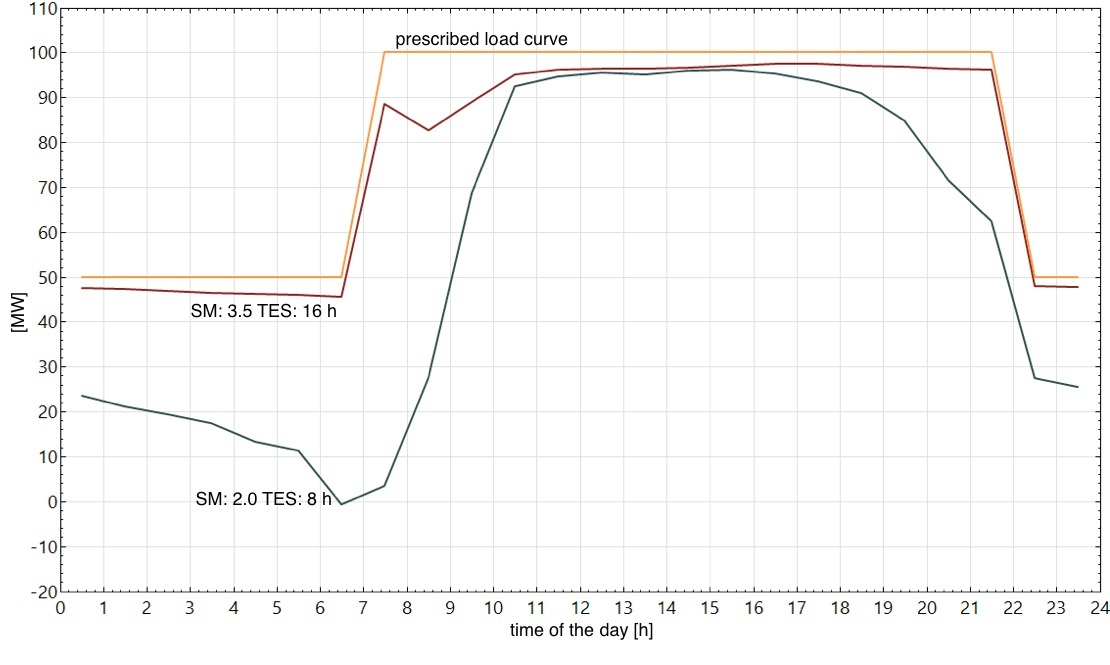
\includegraphics[width=0.8\linewidth]{FIG/CR_annual_profil}
\caption[Annual average load profile of selected CR power plant configurations.]{Annual average load profile of selected CR power plant configurations.}\label{CR_annual_profil}
\end{figure}

%Figure~\ref{CR_annual_profil} shows the annual load curve covering of the above mentioned CR power plant high and low configurations with the prescribed load curve. The Figure shows, that the CR power plant using a SM of 3.5 and \SI{16}{h} of TES for the configuration can cover almost at any time of the year the prescribed load curve. The decreasing of the supplied electricity 8:00 leads from the winter duration and will be shown in the following. The lower CR power plant configuration can just cover between 11:00 and 17:00 almost the same amount electricity during the year than the high configuration. In the morning times between 6:00 and 7:00 the energy production is coming to standstill the whole year. The results of all annual average load profiles can be found in Appendix~\ref{all_load_profile}.

Figure~\ref{CR_annual_profil} shows the annual load curve covering of the above mentioned CR configurations with the prescribed load curve. The CR plant using a SM of 3.5 and \SI{16}{h} of TES can cover the prescribed load curve at almost at any time of the year. Between 11:00 and 17:00, the smaller CR power plant configuration can almost cover as much load as the larger configuration. The results of all annual average load profiles can be found in Appendix~\ref{all_load_profile}.

%At this point it might be necessary to remind, that it is just the electricity used for the annual load covering as well as for the LCOE calculation which is actually supplied at the requested time step. So the electricity which is overproduced at any time of the year is not considered. This can also be seen in Figure~\ref{CR_winter_load}. 
Only electricity used for the annual load covering as well as for the LCOE calculation is actually supplied at the requested time step. Electricity which is overproduced at any time of the year is not considered. 

\begin{figure}[htbp]  
\centering
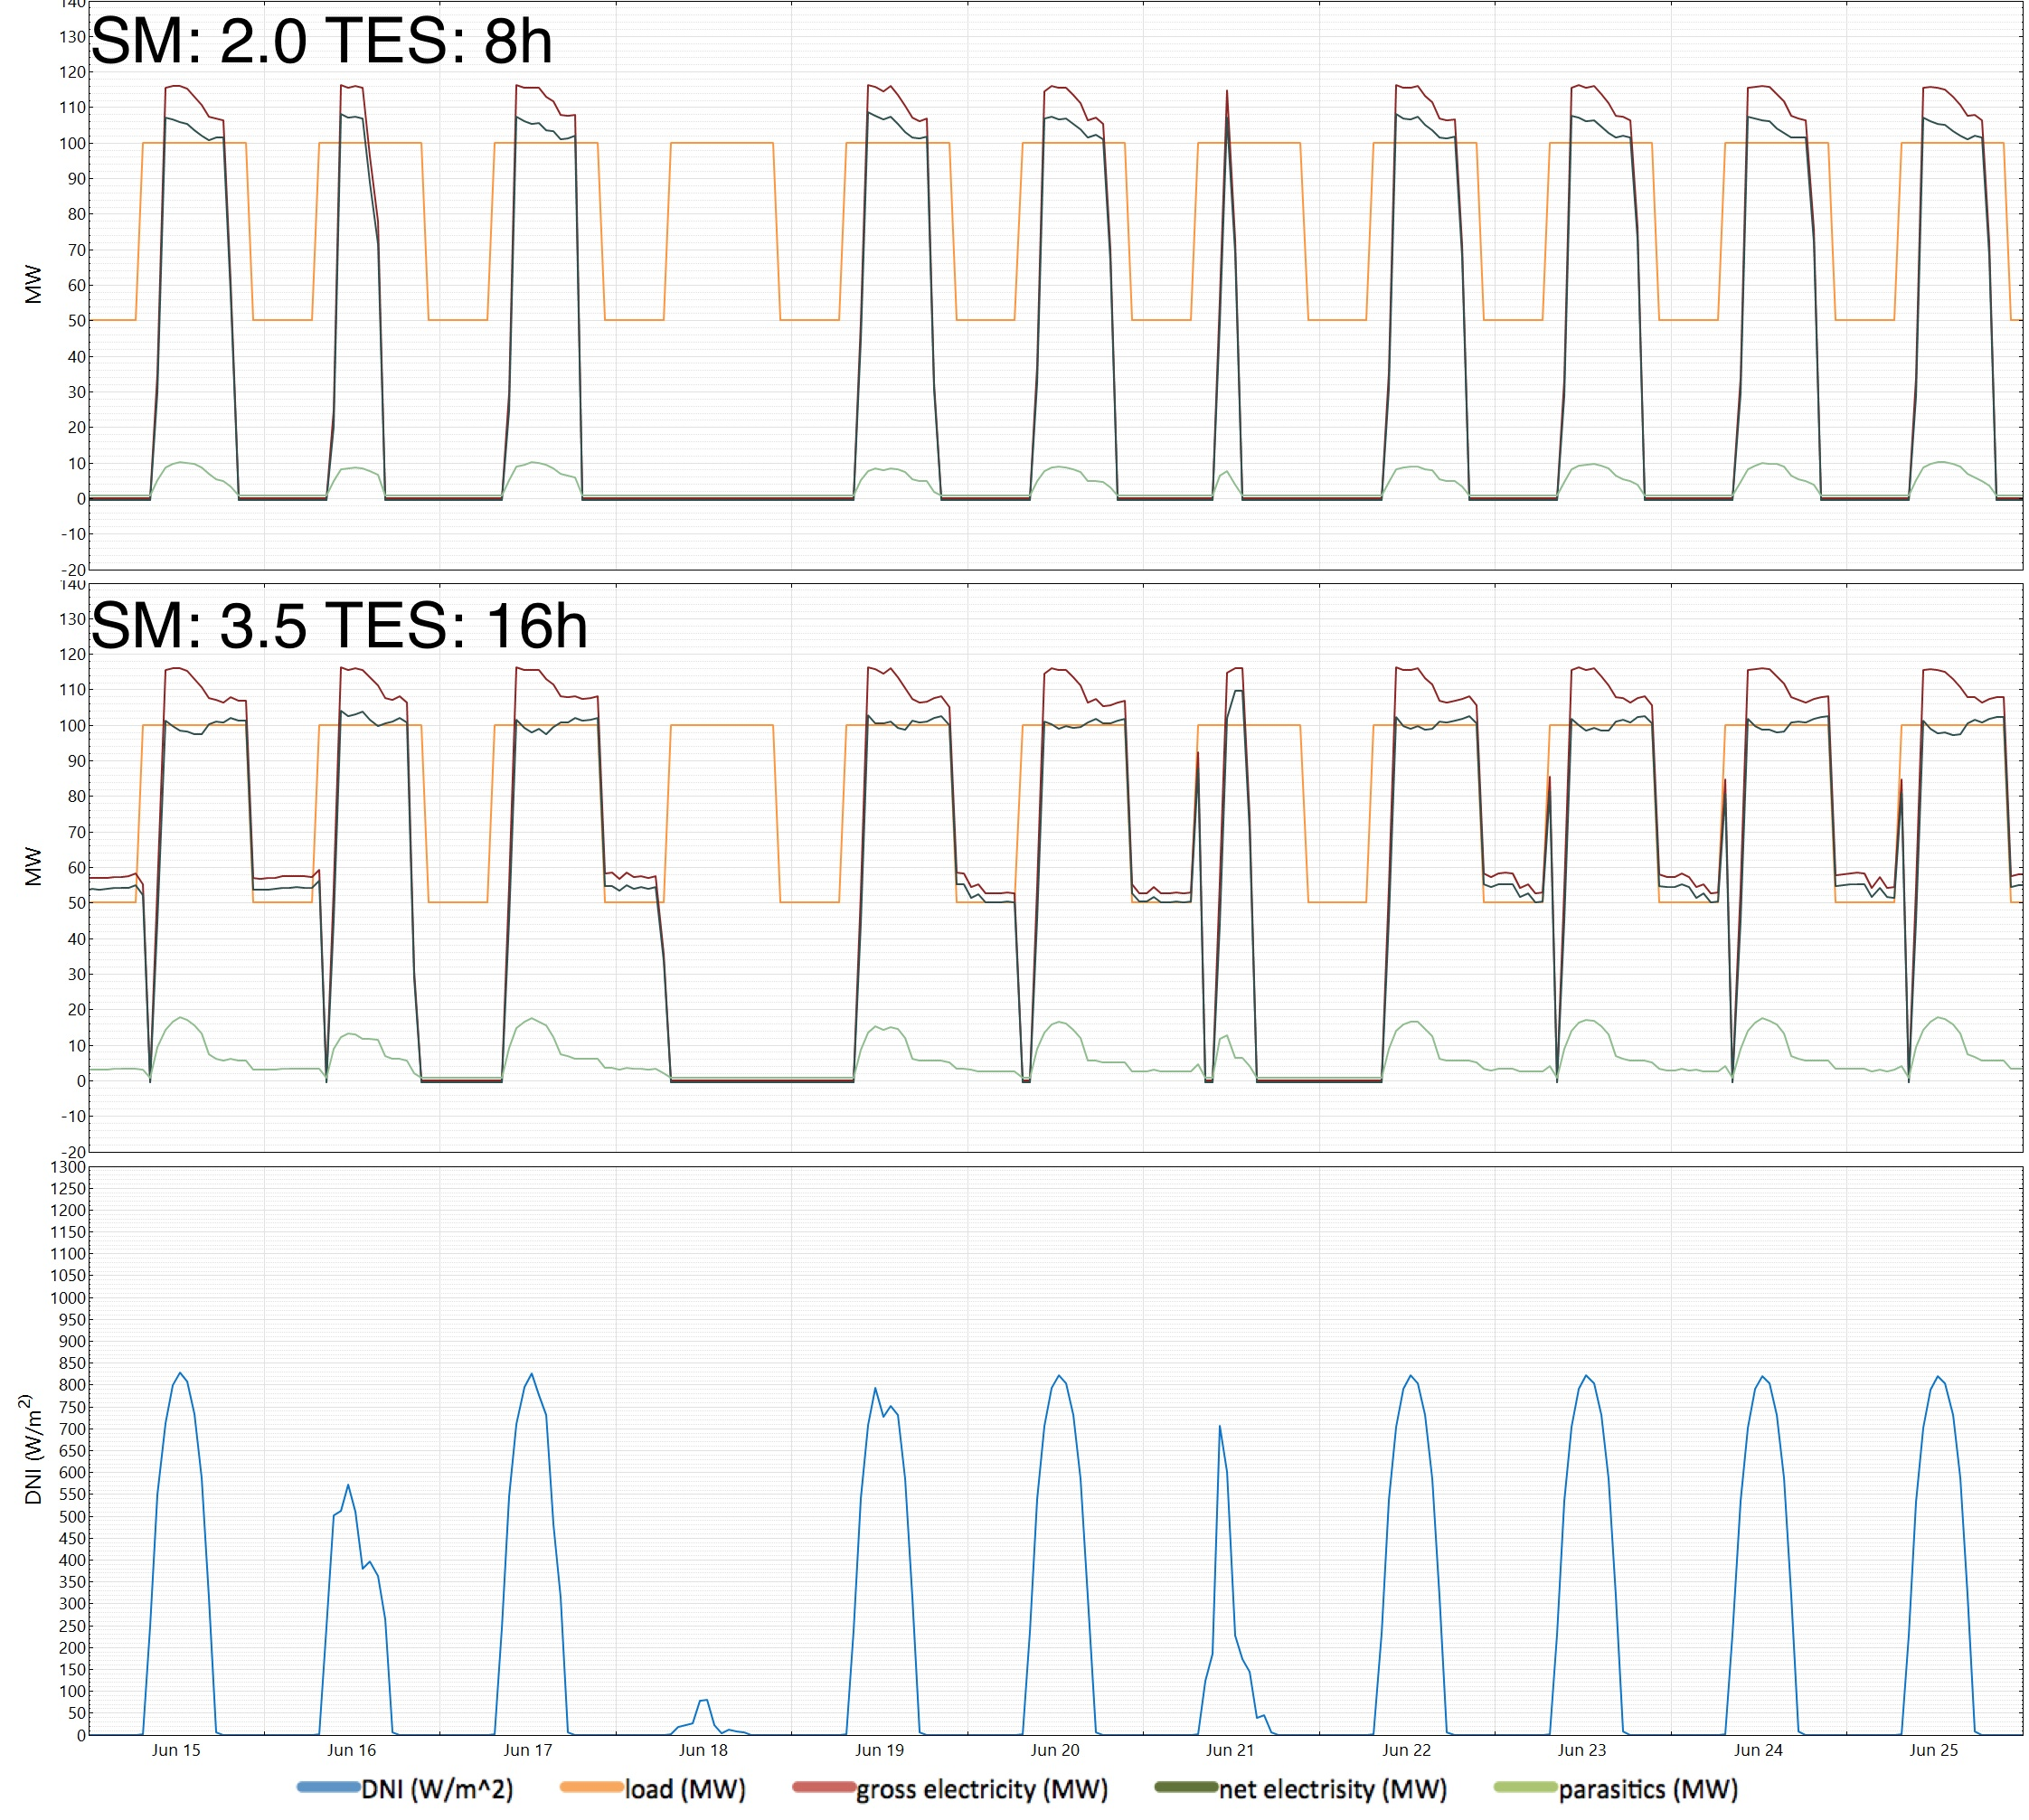
\includegraphics[width=1\linewidth]{FIG/CR_winter_load}
\caption[CR load profile around the northern solstice (15. June - 25. June).]{CR load profile around the northern solstice (15. June - 25. June).}\label{CR_winter_load}
\end{figure}
%This figure shows exemplary the load curve behavior of the CR power plants during the time with the least hours of sunlight during a day of the year. The DNI is around \SI{830}{\watt\per\square\metre} in peak times at these days and there are also days with less or almost no direct irradiance. As mentioned, it can be seen that the net electricity production is in both cases at some times across the prescribed load curve and is not consulted further. This reaches mainly from the described dispatch control matrix from Figure~\ref{CR_turbineoutput} on Page~\pageref{CR_turbineoutput} to control the turbine output. This is not accurate at all to follow a specific load exactly during each day of the year. 
Figure~\ref{CR_winter_load} shows the load curve behaviour of the CR power plants on the days with the fewest hours of sunlight. The DNI is around \SI{830}{\watt\per\square\metre} in peak times on these days and there are also days with less or almost no direct irradiance. Net electricity production is in both cases beyond the prescribed load curve at certain times; this excess is ignored. This results from the dispatch control matrix from Figure~\ref{CR_turbineoutput}, page~\pageref{CR_turbineoutput} which controls the turbine output, and is not realistic.
% Ich verstehe nicht, was du hier sagen wolltest. Ich habe versucht, den Satz zu retten.

%However, Figure~\ref{CR_winter_load} mainly shows the load curve behavior of the CR power plants in low and high configuration. At a SM of \si{2.0} with \SI{8}{h} of TES the power plant can't produce enough power during the day to fill up the TES for generating power during the night. Compared to that, the CR power plant with a SM of \si{3.5} and \SI{16}{h} of TES can almost anytime generate electricity over the whole night. But with the rising load in the morning hours the energy production stops due to the empty storage. 
Figure~\ref{CR_winter_load} shows the load curve behaviour of the CR power plants in small and large configurations. At a SM of \si{2.0} with \SI{8}{h} of TES, the plant cannot deliver sufficient power during the day to charge the TES. By contrast, a CR power plant with a SM of \si{3.5} and \SI{16}{h} of TES can generate electricity over the whole night. However, as load rises in the morning hours, the electricity production is interrupted due to empty storage. 

\begin{figure}[htbp]  
\centering
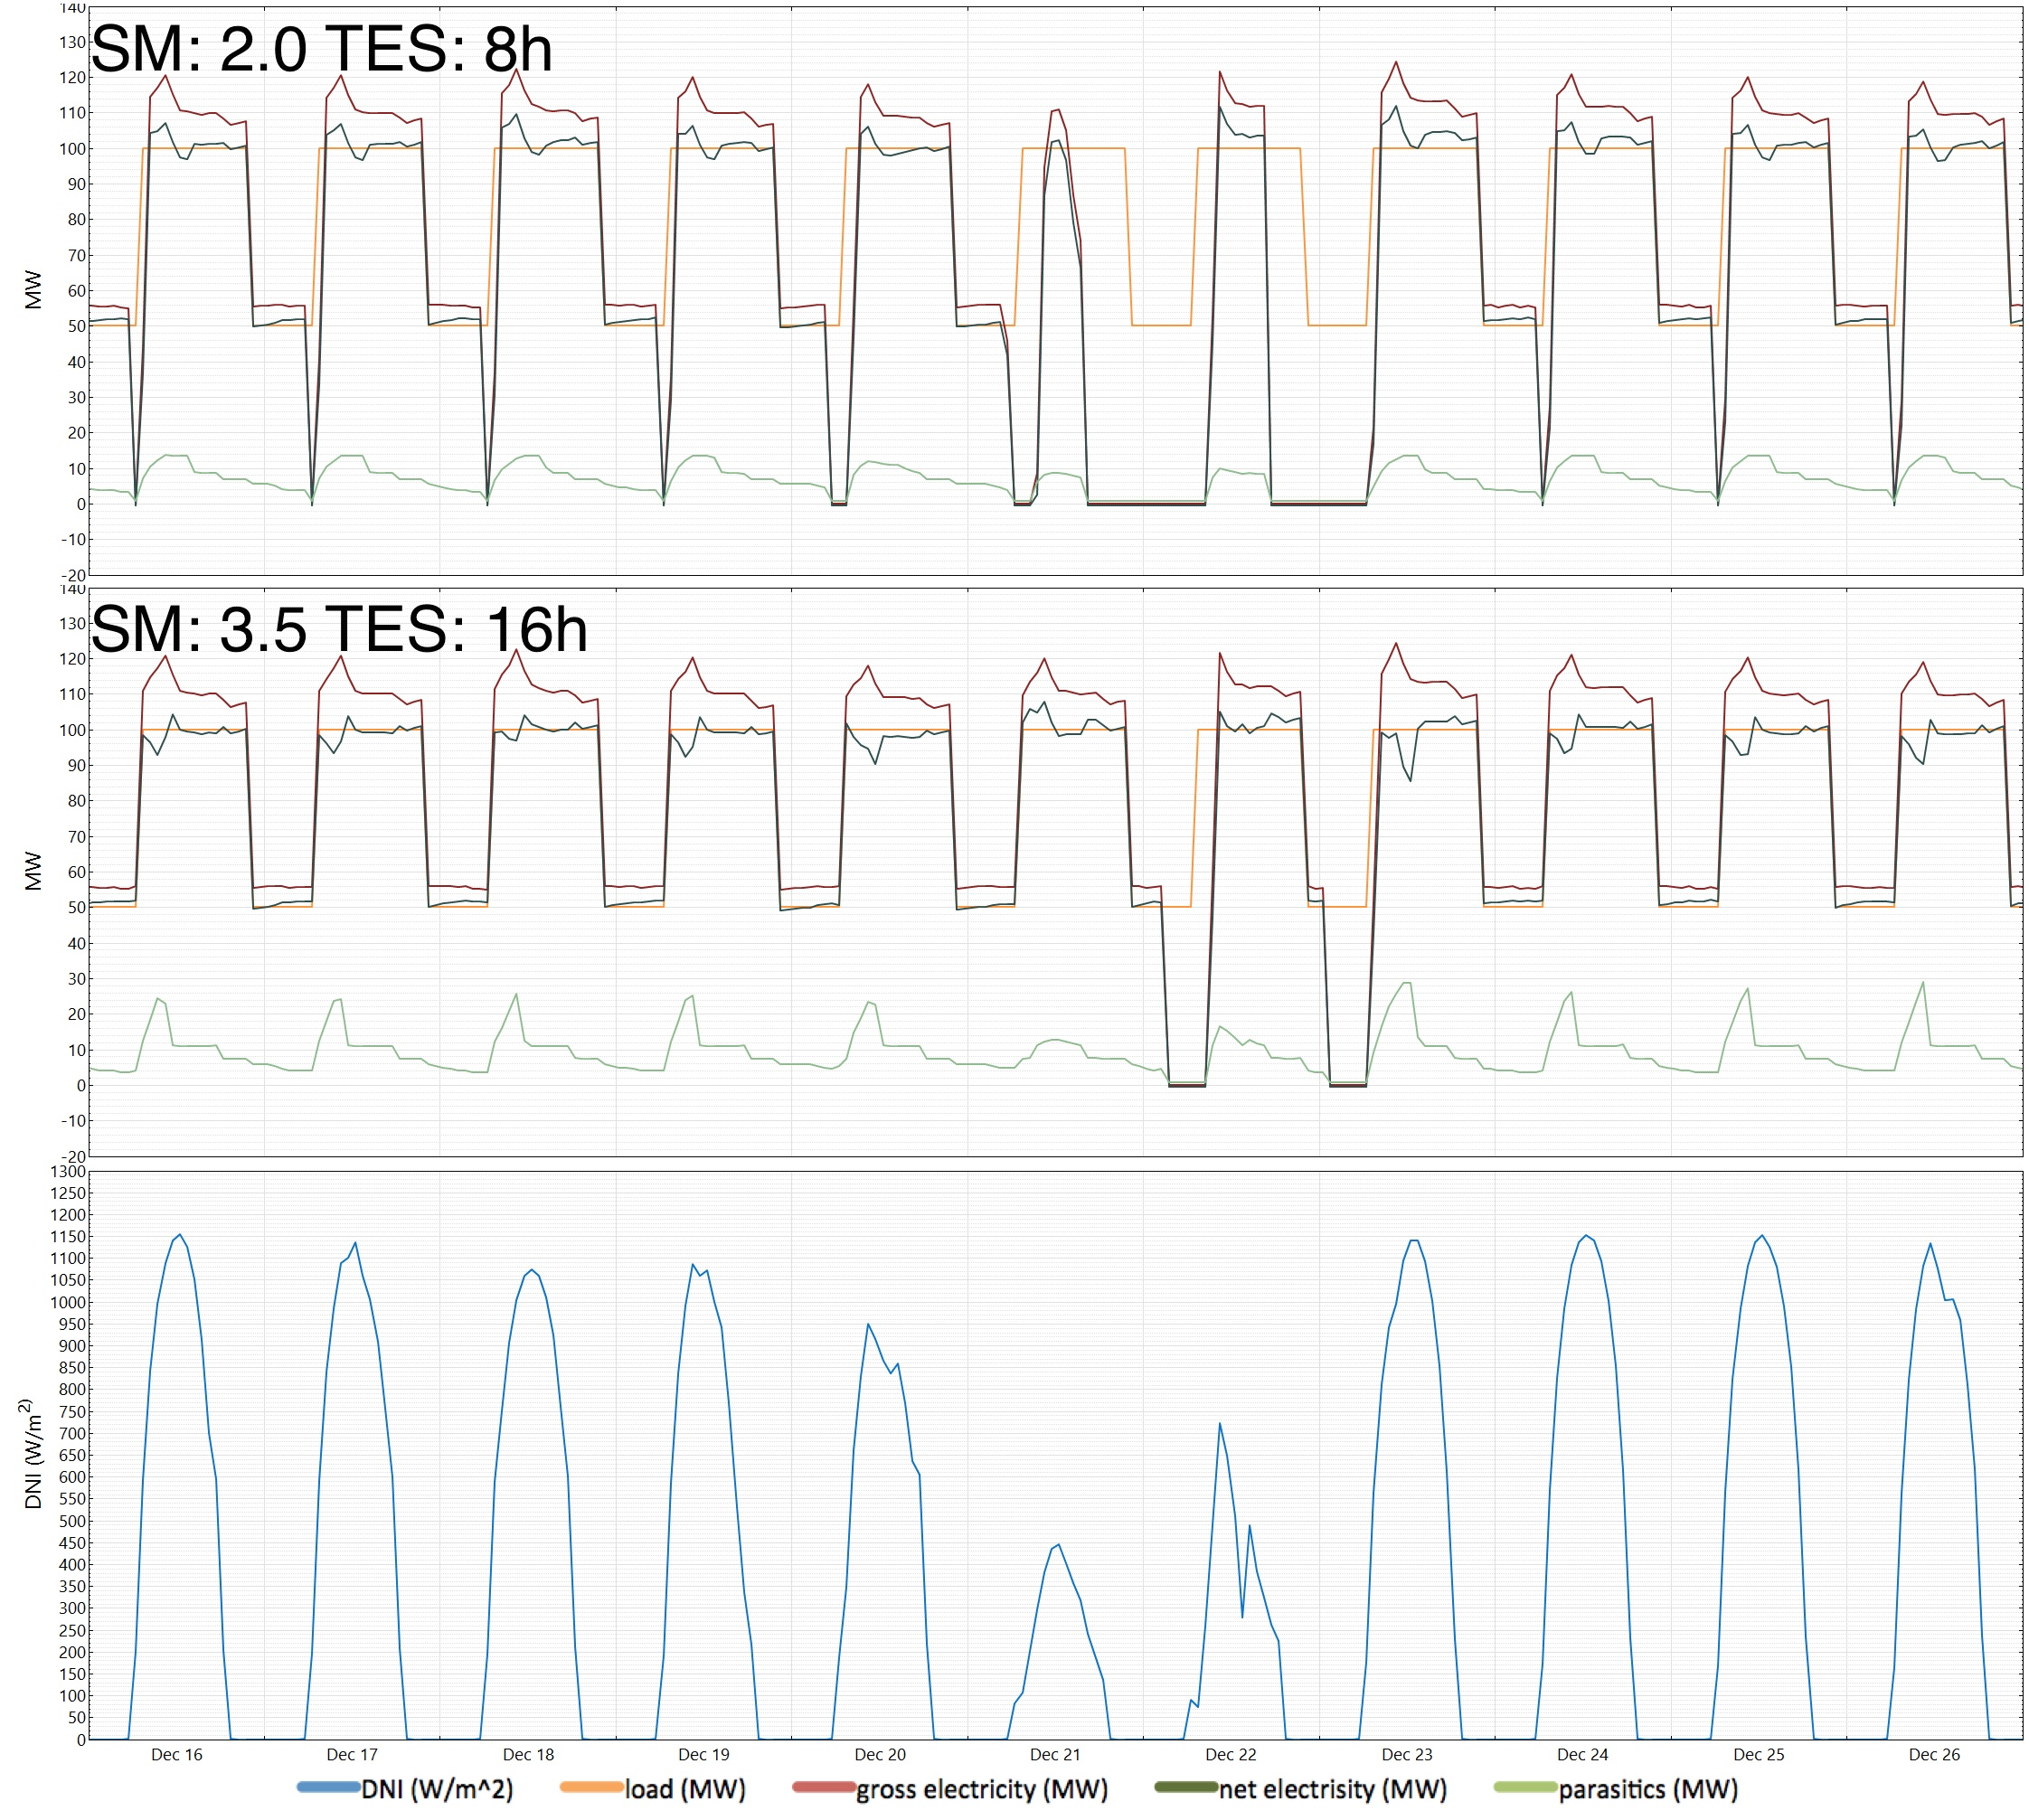
\includegraphics[width=1\linewidth]{FIG/CR_summer_load}
\caption[CR load profile around the southern solstice (16. December - 26. December).]{CR load profile around the southern solstice (16. December - 26. December).}\label{CR_summer_load}
\end{figure}
%This leads also to the above mentioned decreasing in supply at \SI{8}{am} in the annual average load profile. The difference between the gross and net electricity production is coming from the parasitic consume within the power plant.

This leads also the drop in supply at \SI{8}{am} in the annual average load profile. The difference between gross and net electricity production comes from parasitic consumption within the plant.

%Figure~\ref{CR_summer_load} describes the load behavior of the  same power plants during the longest days of the year. It is clearly to see, that the irradiation is higher and longer during the days compare to the winter solstice. The peaks of DNI are about 1~\SI{150}{\watt\per\square\metre} during that days. At a SM of 2.0 and \SI{8}{h} of TES the CR power plant is not able to follow the prescribed electricity load over the whole day. It's coming to standstill between 6 and \SI{7}{am} at least. Therefrom also the annual average load profile is coming to stand still at these time of the day. The CR power plant with a SM of 3.5 and \SI{16}{h} of TES can follow the prescribed load mostly without any problems. Outstanding for the high productivity of the plant configuration is the electricity output while having low direct irradiance. At the 21. of December the plant can supply almost the whole prescribed load using reserves from the TES.
Figure~\ref{CR_summer_load} shows the behaviour of the same plants during the longest days of the year. The peaks of DNI are about \SI{1150}{\watt\per\square\metre} during this period. At a SM of 2.0 and \SI{8}{h} of TES, the plant is not able to follow the prescribed electricity load over the whole day, dropping between 6 and \SI{7}{am}. The plant with a SM of 3.5 and \SI{16}{h} of TES can follow the prescribed load without difficulty. Of note is the output when there is low direct irradiance. On 21. December, the plant can supply almost the entire prescribed load using reserves from the TES.

%A detailed look to the parasitic behaviors of the CR power plant with a SM of \si{3.5} and \SI{16}{h} of TES reveals a strong decreasing after a moderate increasing during the midday. This happens when the storage is full loaded and the steam turbine don't need more power. At this point a specified amount of heliostats defocusing the receiver and the power of the receivers HTF pump is getting reduced. 

A detailed look at the parasitic behaviour of the CR power plant with a SM of \si{3.5} and \SI{16}{h} of TES reveals a strong decrease after a moderate increase during midday. This happens when the storage is fully charged and the steam turbine does not need more power. At this point, a specified number of heliostats defocus from the receiver and the power of the receiver's HTF pump is reduced. 

\begin{figure}[!htbp]
        \centering   
        \begin{subfigure}[b]{0.65\textwidth}
                \centering
                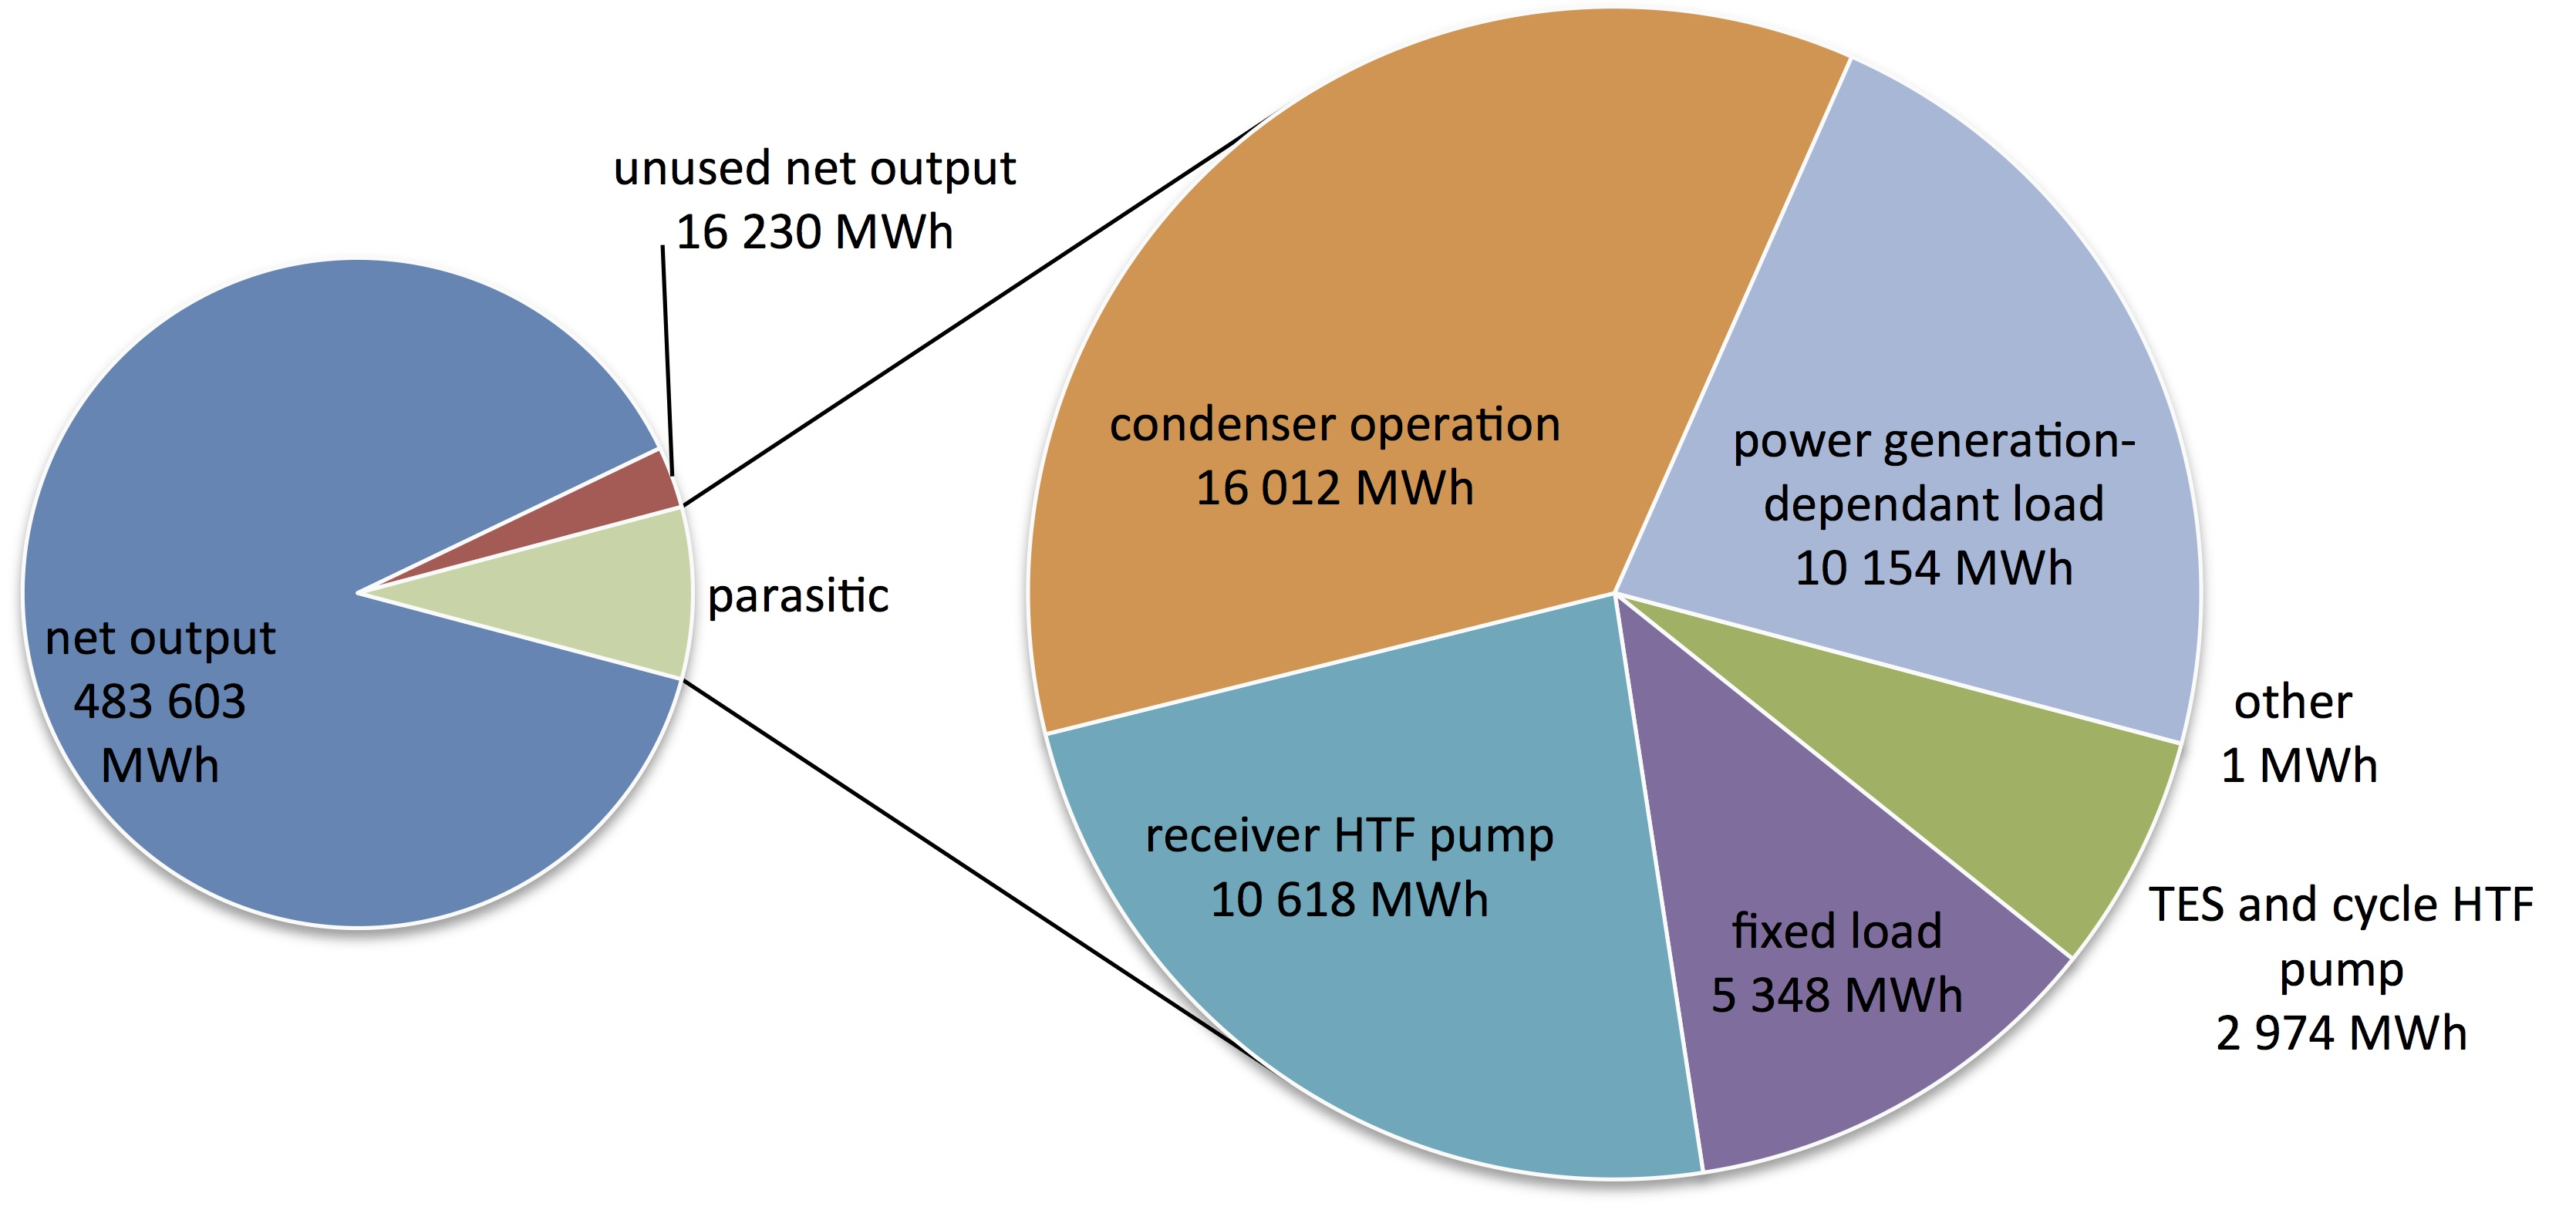
\includegraphics[width=1\textwidth]{FIG/CR_parasitics_low}
                \caption{SM: 2.0 TES: 8 h}\label{CR_parasitics_low}
        \end{subfigure}
\par\medskip % Linebreak              
        \begin{subfigure}[b]{0.65\textwidth}
                \centering
                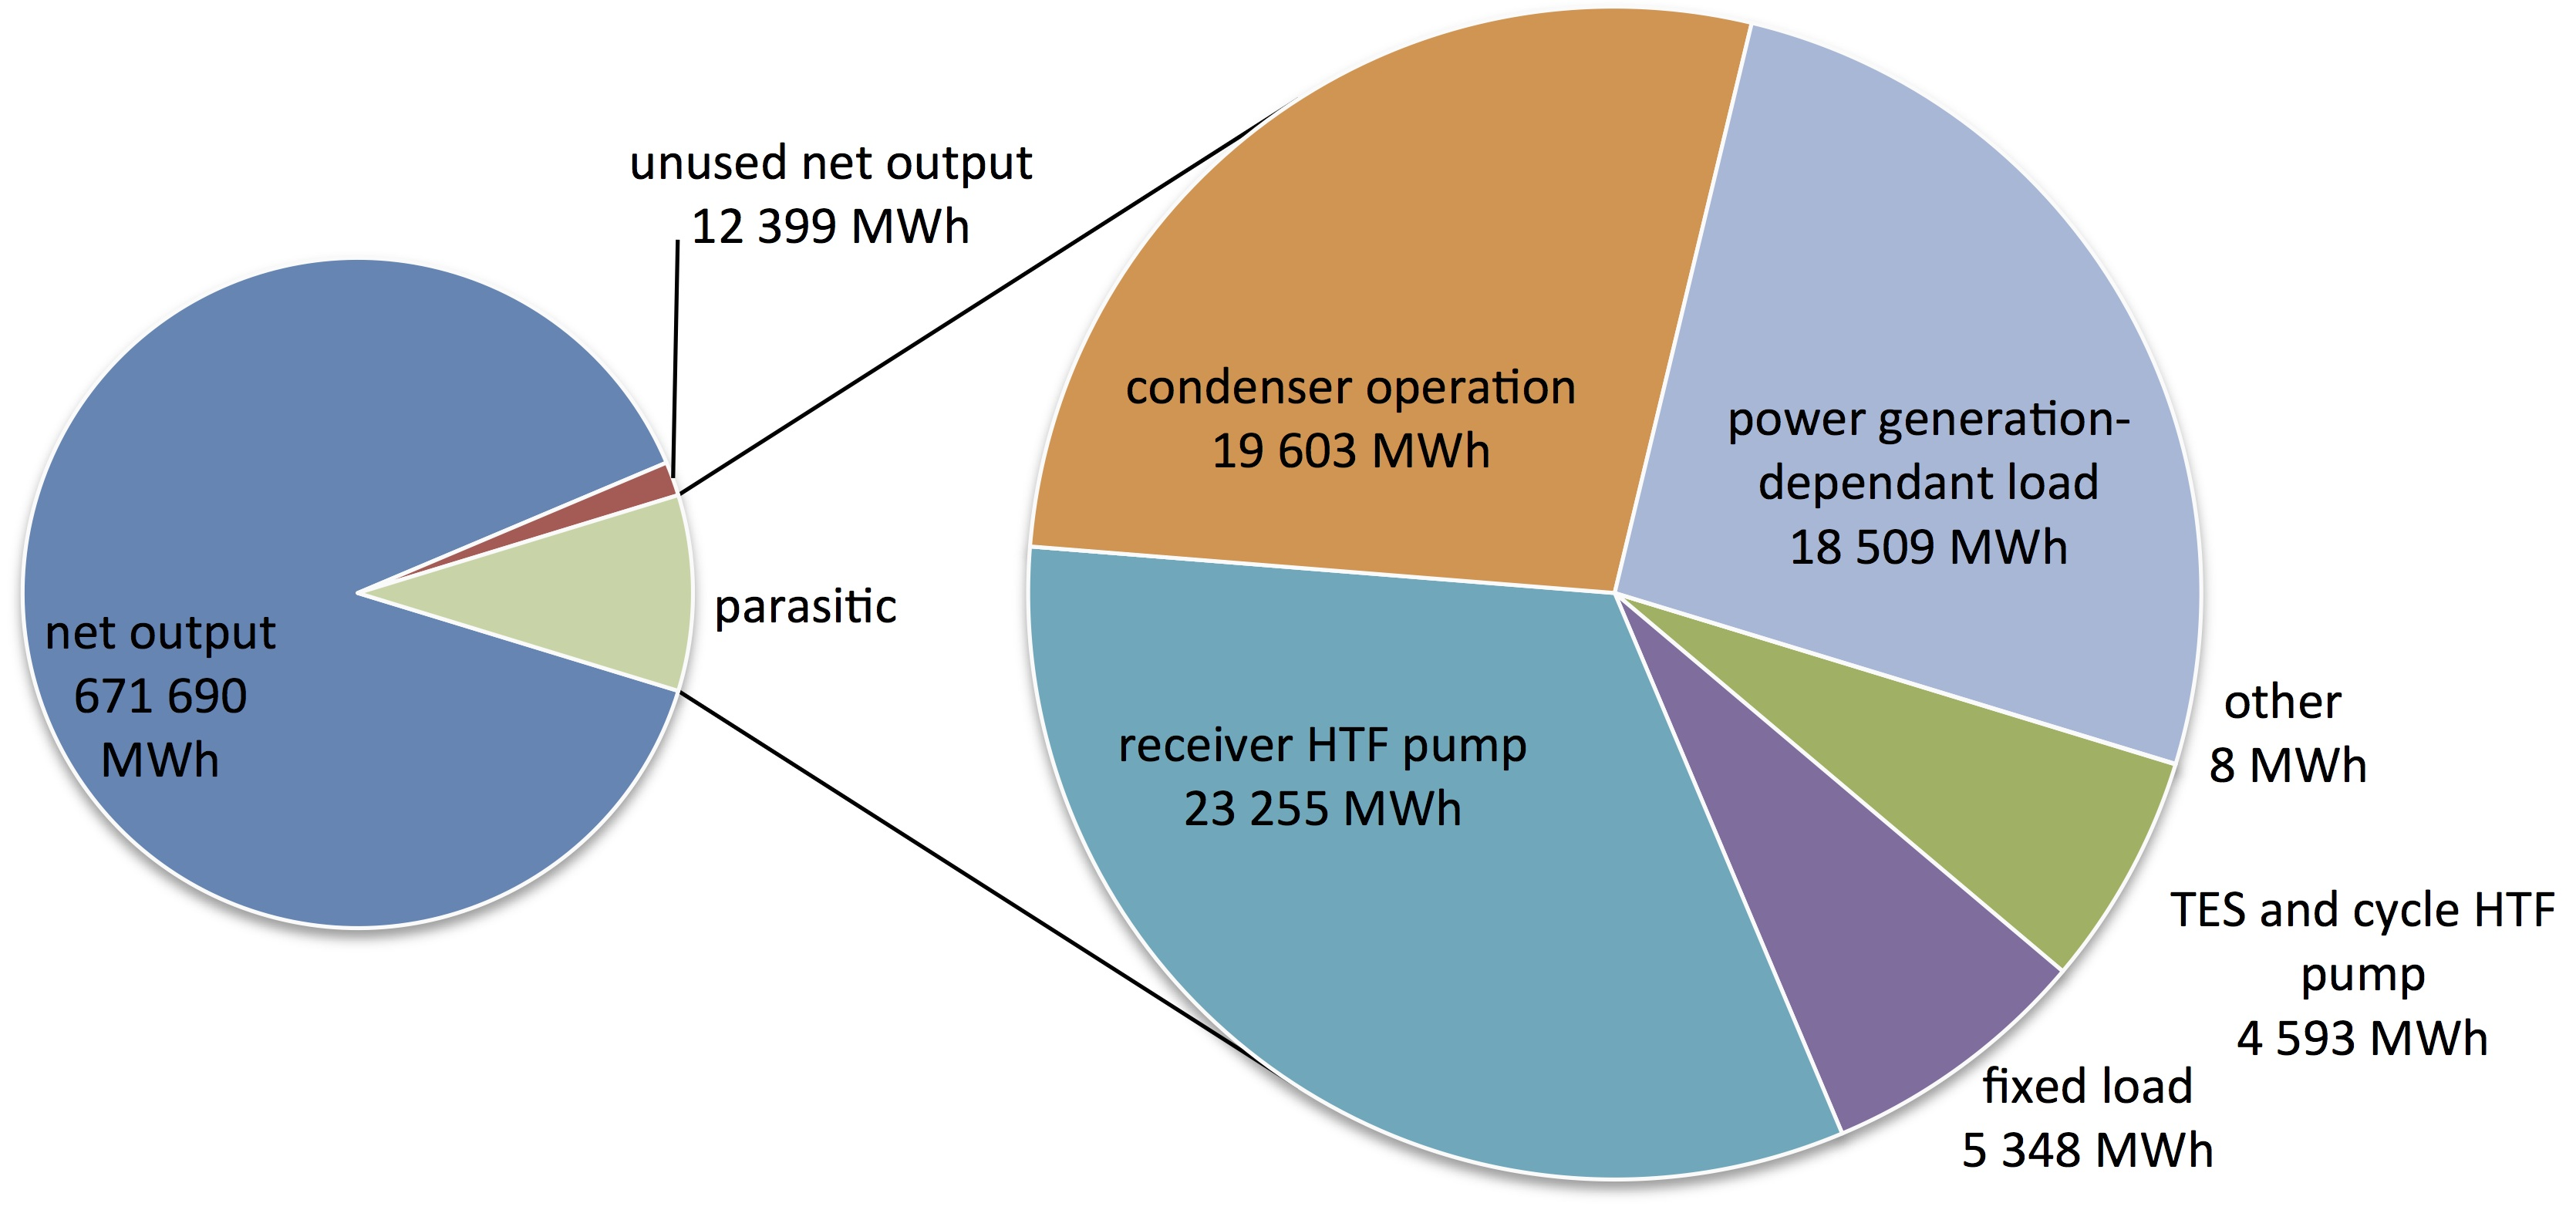
\includegraphics[width=1\textwidth]{FIG/CR_parasitics_high}
                \caption{SM: 3.5 TES: 16 h}\label{CR_parasitics_high}
        \end{subfigure}
        \caption[Share of annual gross energy output of selected CR power plant configurations.]{Share of annual gross energy output of selected CR power plant configurations.}\label{CR_parasitics}
\end{figure}
%The parasitic load is composed from various electrical loads of the power plant, namely pumping loads, cooling loads, fixed loads and loads depending from the power generation. The share of these electrical parasitic loads and the total share of the gross energy output of the selected CR power plans can be seen in Figure~\ref{CR_parasitics}. The share of the net energy production out of the gross energy production is about 90~\%. The unused net energy output share of all simulated CR power plants is between 1.6 and 3.2~\% and went not into the LCOE calculation.
The parasitic load is composed of various electrical loads of the power plant, namely pumping loads, cooling loads, fixed loads and loads depending on power generation (Figure~\ref{CR_parasitics}). The share of net energy production from gross energy production is about \SI{90}{\percent}. The unused net energy output share of all simulated CR power plants is between \num{1.6} and \SI{3.2}{\percent} and was not included in the LCOE calculation.

%Figure~\ref{CR_parasitics_low} shows, that the net outputs share of the lowest CR power plant configuration is about \SI{483.60}{GWh}.  The total sum of the annual prescribed load is \SI{711.75}{GWh}. So the power plant covers the prescribed load for 67.9~\%. The net outputs share of the highest CR power plant configuration from Figure~\ref{CR_parasitics_high} is \SI{671.69}{GWh} and is covering the prescribed load for 94.4~\% over the year.
The share of net outputs of the smallest CR power plant configuration is \SI{483.60}{GWh} (Figure~\ref{CR_parasitics_low}). The total sum of the annual prescribed load is \SI{711.75}{GWh}. The plant covers \SI{67.9}{\percent} of the prescribed load. The net outputs share of the largest CR power plant configuration is \SI{671.69}{GWh} (from Figure~\ref{CR_parasitics_high}) and this covers the prescribed load to \SI{94.4}{\percent} over the year.

%Figure~\ref{CR_LCCF} summarizes the results of the load curve covering for all simulated CR configurations. The chart shows that at a SM of 2.0 all TES variations besides \SI{8}{h} a covering more than 70~\% of the prescribed load. At a SM of 2.5 the and a TES about \SI{10}{h} the results showed over 80~\% load covering. A load curve covering of about 90~\% is reached at a SM of 3.0 and more than \SI{14}{h} of TES. The configuration with a \SI{12}{h} TES reaches just 89.1~\% at a SM of 3.0. 

Figure~\ref{CR_LCCF} summarizes the results of the load curve covering for all simulated CR configurations.

% Du solltest die Schlussfolgerung klarer machen. Hier leierst du lediglich den Bildinhalt runter, das ist nicht gut. Die Arbeit ist bereits lang genug. Kurz und bündig lautet die Devise! Weniger ist mehr!

\begin{figure}[htbp]  
\centering
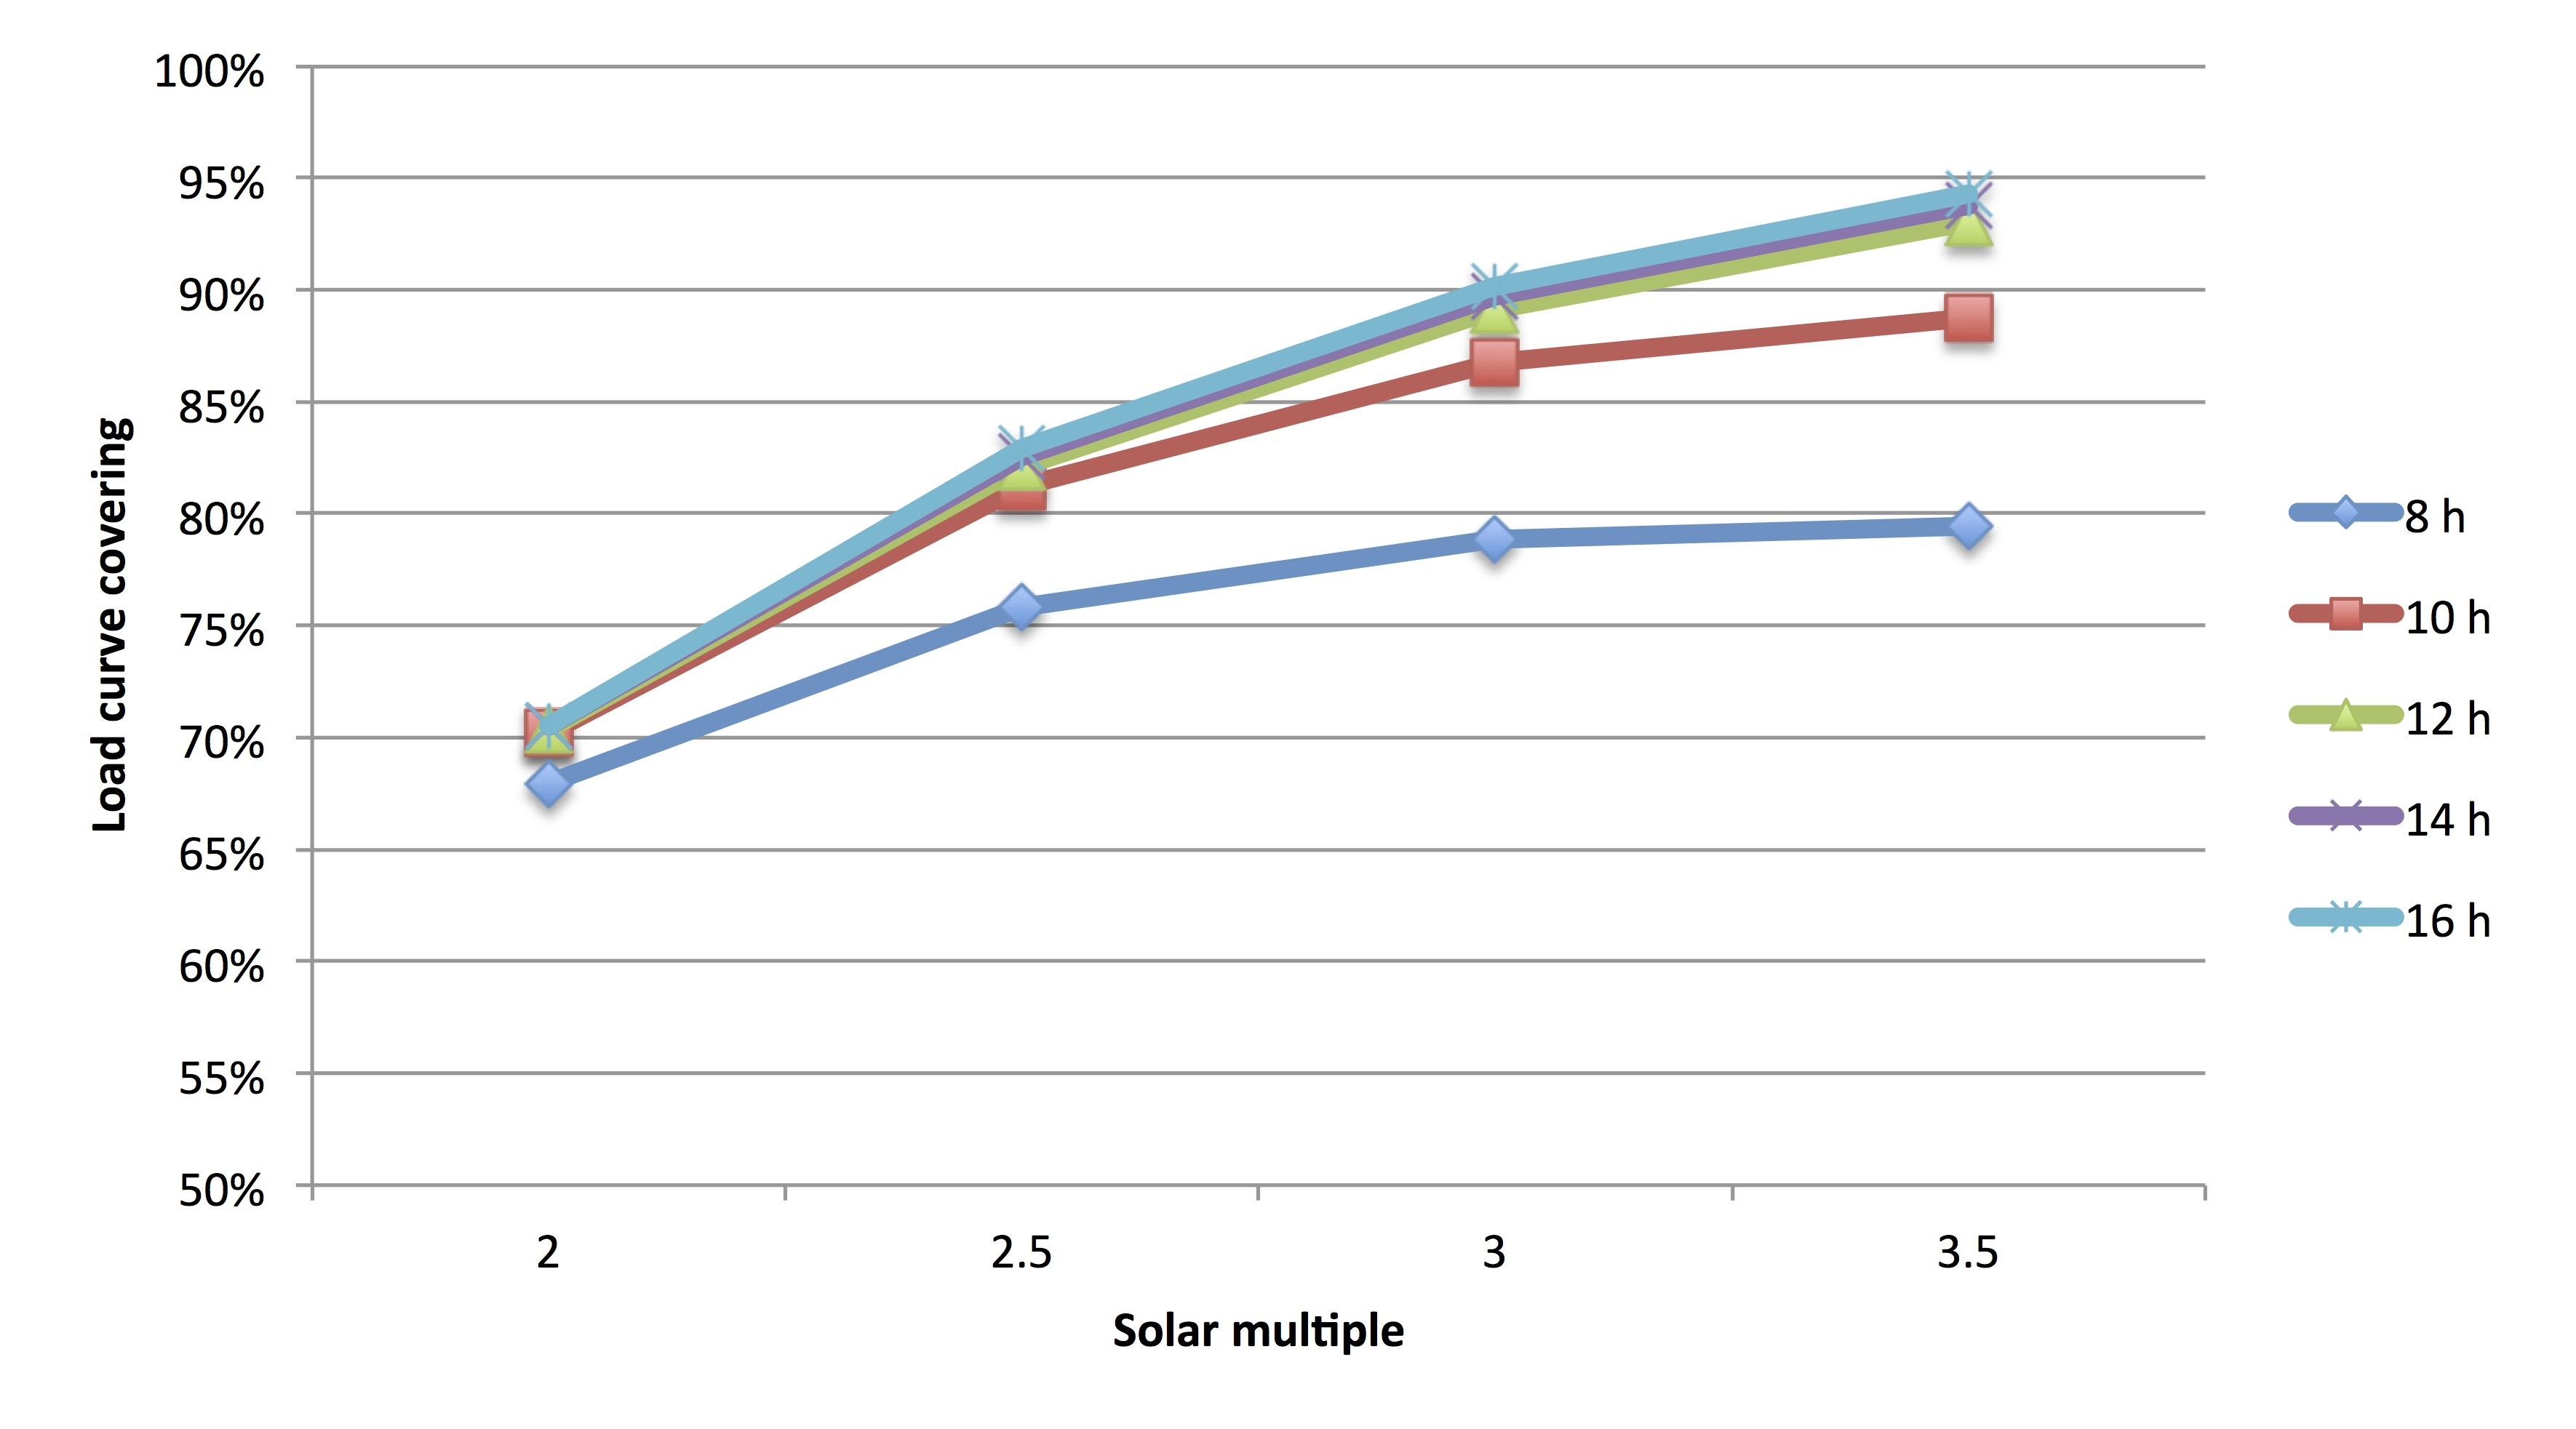
\includegraphics[width=1\linewidth]{FIG/CR_LCCF}
\caption[Load curve coverage of simulated CR systems.]{Load curve coverage of simulated CR systems.}\label{CR_LCCF}
\end{figure}
%The results of the load curve covering shows that there is no appreciable difference between the \SIlist{12;14;16}{h} of TES. At a SM of 3.5 the difference is just \SI{1.4}{\percent} load curve covering between \SIlist{12;16}{h} of TES. There is just a addition of \SI{0.6}{\percent} for the \SI{8}{h} TES and the SM 3.0 to 3.5 configurations.

The results of the load curve coverage analysis show that there is no appreciable difference between the \SIlist{12;14;16}{h} of TES. At a SM of 3.5, the difference between \SIlist{12;16}{h} of TES is a mere \SI{1.4}{\percent} coverage. Solar multiples beyond 3 have a negligible impact on the \SI{8}{h} TES configuration.

\subsubsection{Levelized costs of electricity}
%The results of the calculation shows that the lowest LCOE of \SI{142.31}{USD/MWh} is reached at a SM of 2.0 and \SI{10}{h} of TES and is just  marginal cheaper then using \SI{8}{h} of TES with a LCOE of \SI{143.04}{USD/MWh}. The LCOE addition from SM 2.0 to 2.5 is goes minimal up to \SI{138.25}{USD/MWh} for \SI{10}{h} of TES. The highest LCOE result of the simulated configurations is \SI{185.20}{USD/MWh} at a SM of 3.5 and \SI{8}{h} of TES. 

The results of the LCOE calculation for the simulated CR configurations can be seen in Figure~\ref{CR_LCOE}. They are calculated using the finacial input parameter in Table~\ref{tbl: CRFinance} and the simplified method (see Appendix~\ref{ChapterLCOE}, see \pageref{ChapterLCOE}). 

The LCOE curve behaviour for 12, 14 and \SI{16}{h} TES configurations for all SM is similar.

\begin{figure}[htbp]  
\centering
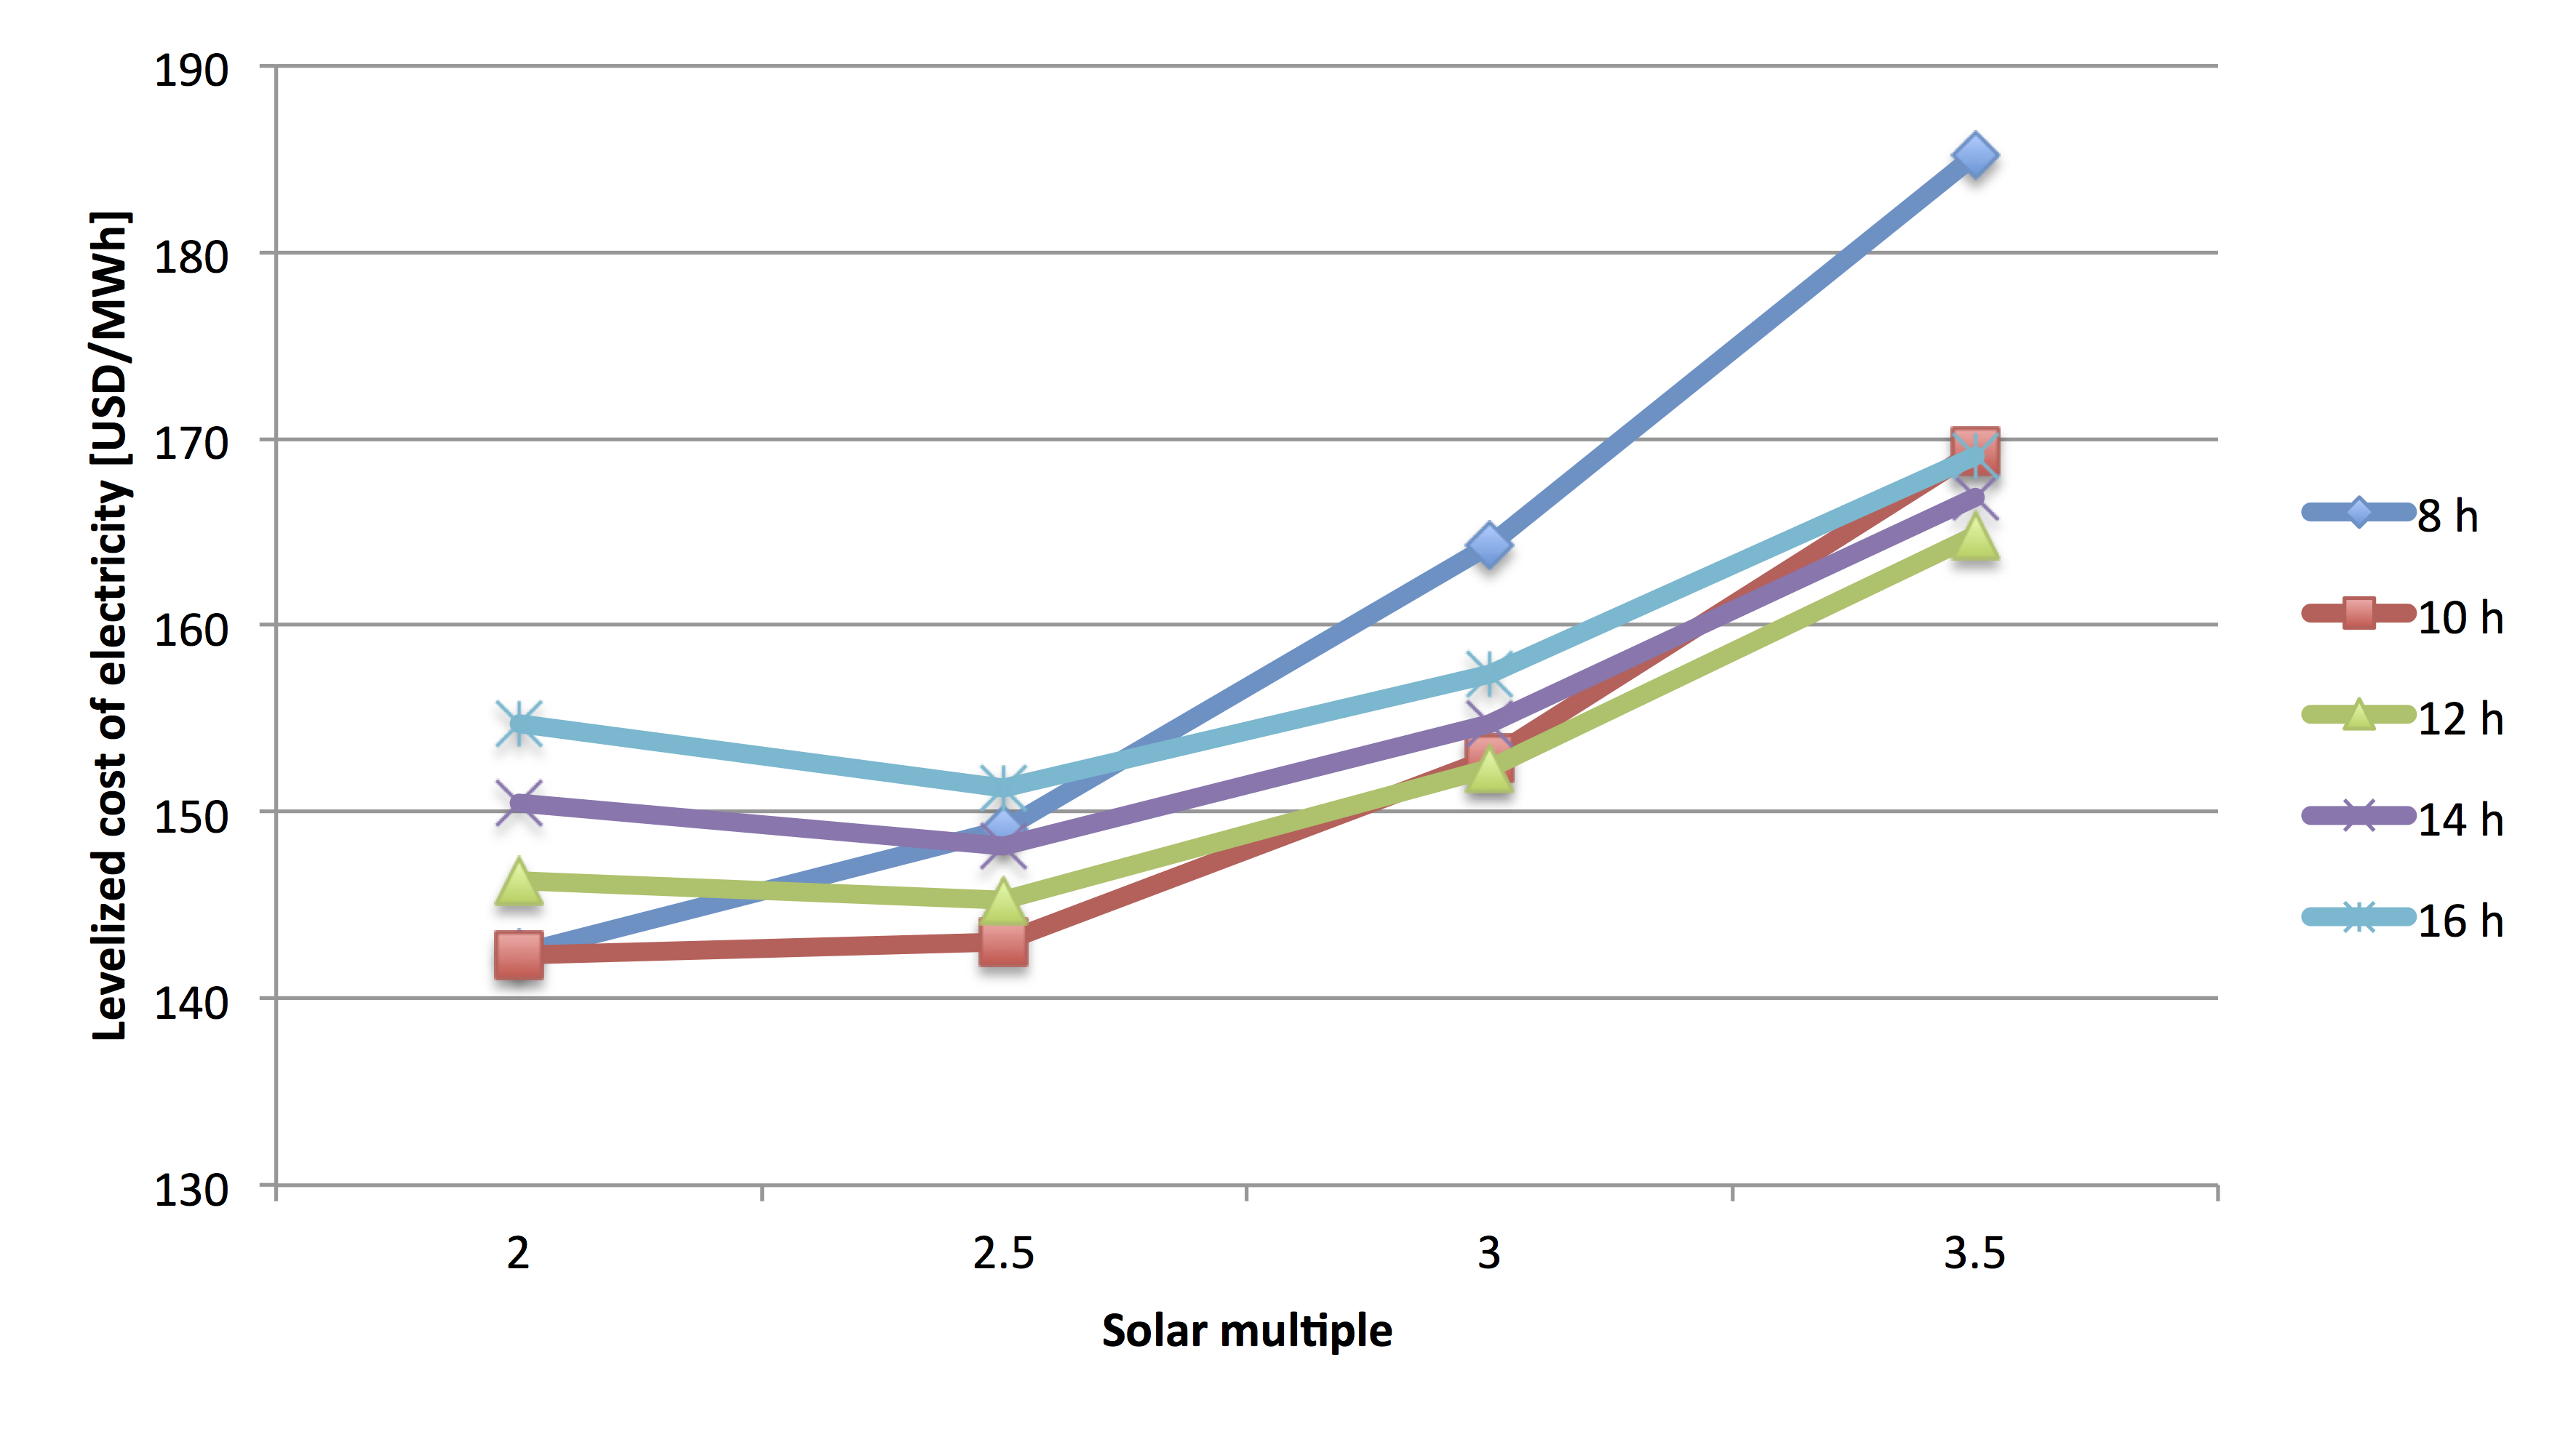
\includegraphics[width=1\linewidth]{FIG/CR_LCOE}
\caption[LCOE calculation results for CR simulation.]{LCOE calculation results for CR simulation.}\label{CR_LCOE}
\end{figure}

%When comprising the results of the load curve covering with the LCOE calculation the lowest LCOE for reaching the target of 90~\% is the configuration of a SM of 3.0 and \SI{14}{h} of TES. The LCOE for these configuration is \SI{154.75}{USD/MWh}. 
When comparing the results of the load curve coverage analysis with the LCOE, the lowest LCOE for the \SI{90}{\percent} target is at a SM of 3.0 and \SI{14}{h} of TES. The LCOE for this configuration is \SI{154.75}{USD/MWh}.

%For reaching 80~\% of the prescribed load curve the lowest LCOE is \SI{143.04}{USD/MWh} using a SM of 2.5 and \SI{10}{h} of TES. The lowest LCOE for covering 70~\% of the prescribed load curve is also the lowest LCOE of all and is mentioned above.
At a coverage of \SI{80}{\percent}, the lowest LCOE is \SI{143.04}{USD/MWh} at a SM of 2.5 and \SI{10}{h} of TES. The lowest LCOE for \SI{70}{\percent} coverage is the minimum, \SI{138.25}{USD/MWh}, at SM 2.0 to 2.5 and \SI{10}{h} of TES.